\documentclass[fignum,nobf,doc,noapacite]{apa}
\newtheorem{lemma}{Lemma}
\newcommand{\pd}[2]{\frac{\partial#1}{\partial#2}}
\newcommand{\R}{R}
\def\citeapos#1{\citeauthor{#1}'s (\citeyear{#1})}

\usepackage{eurosym}
\usepackage{graphicx}
\usepackage{amsfonts}
\usepackage{amsbsy}
\usepackage{listings}
\usepackage{setspace}
\usepackage{pdfcomment}
\usepackage{subcaption}
\usepackage{pdfpages}		% to include the full-page plot
\usepackage{authblk}		% for mulitple authors with different affiliations

\usepackage[american]{babel}
\usepackage{csquotes}
\usepackage[style=apa,natbib=true, backend=biber]{biblatex}
\DeclareLanguageMapping{american}{american-apa}


\usepackage[T1]{fontenc}
\usepackage[sc]{mathpazo}
\usepackage{color}
\linespread{1.05}         % Palatino needs more leading (space between lines)

\bibliography{bibfile}

\abstract{Experiments suggest that there is a strong tendency to verbally recode visually-presented information, and that in some cases verbal recoding can boost memory performance.  According to multi-component models of working memory, memory performance is increased because task-relevant information is maintained in two codes. The possibility of dual encoding is problematic if the goal is to measure capacity for visual information exclusively. This is why articulatory suppression is typically used with visual change detection tasks specifically to prevent verbalization of visual stimuli. We present evidence from a large experiment that suggests that articulatory suppression has no discernable effect on performance in a visual change-detection task. Neither a descriptive nor a state-trace analysis revealed any complex relationship between suppression, presentation type, and performance. There is no evidence that verbal recoding was a strategy used by the participants in this task. We conclude that in typical visual change detection experiments, pre-cautionary articulatory suppression is unnecessary.}


\rightheader{}
\shorttitle{}

\leftheader{}


\title{Opportunity for verbalization does not improve visual change detection performance: A state-trace analysis.}

\author[1]{Florian Sense}
\author[2]{Candice C. Morey}
\author[3]{Melissa Prince}
\author[4]{Andrew Heathcote}
\author[5]{Richard D. Morey}

\affil[1]{Department of Experimental Psychology \& Department of Psychometrics and Statistics, University of Groningen}
\affil[2]{Department of Psychology, University of Edinburgh}
\affil[3]{School of Psychology, Flinders University, Australia}
\affil[4]{School of Medicine, The University of Tasmania, Australia}
\affil[5]{School of Psychology, Cardiff University}

\lstset{tabsize=2}
\acknowledgements{Please address correspondence to: {\tt f.sense@rug.nl}. The code for all analyses and plots as well as the complete dataset can be found at {\tt https://github.com/fsense/opportunity-verbalization-statetrace}.

We would like to thank Yongqui Cong, Christian Hummeluhr, and Mareike Kirsch for valuable assistance with data collection.}


\begin{document}
\maketitle


\newpage

\section{Introduction}
% !TeX root = sta_paper.tex

During his seminal experiments on human memory, Sperling noticed that many of his participants verbalized and repeated to-be-remembered material during rehearsal, even if the studied material was not aurally presented. \citet{Sperling:1967} pointed out that visual information can be verbalized and many people reported doing so. This reflection confirmed to cognitive psychologists interested in the structure and mechanisms underlying memory that presentation modality likely affects encoding. Like Sperling, they used this insight as a basis for inquiry into the nature of memory representations.

For example, \citet{Murray:1965} showed that saying visually-presented verbal stimuli out loud improves recall performance relative to mouthing them silently. However, this relationship only seems to persist if the visually-presented material can be verbalized effectively (e.g., verbal stimuli, nameable visual images). Attempts to verbalize stimuli that are difficult to describe succinctly and accurately (e.g., faces) might actually harm performance \citep{Schooler:Engstler-Schooler:1990}. \citet{Brandimonte:etal:1992} showed that verbal recoding can be detrimental to a subsequent mental rotation task when the remembered verbal label is not relevant or helpful. What such experiments suggest is that there is a strong tendency to verbally recode visually-presented information, and that in some cases verbal recoding can boost memory performance. This logic is consistent with multi-component models of working memory, which propose that separate short-term memory stores for phonological and visual information can be applied to a short-term memory task \citep{Baddeley:1986}. Naturally, if task-relevant information can be maintained simultaneously in two codes, one would expect memory performance to improve. 

However, the possibility of dual encoding is problematic if the goal is to measure capacity for visual information exclusively. \citet{Levy:1971} suggested a method of preventing such recoding via meaningless concurrent articulation. By repeating irrelvant syllables out loud during presentation and rehearsal of visual information, participants' ability to verbally recode visually-presented stimuli is restricted. This procedure is known as \emph{articulatory suppression} and is commonly used with visual change detection tasks specifically to prevent verbalization of visual stimuli \citep[e.g.][]{Allen:etal:2006, Brockmole:etal:2008, Delvenne:Bruyer:2004, Hollingworth:Rasmussen:2010, Logie:etal:2009, Makovski:Jiang:2008, Makovski:etal:2008, Matsukura:Hollingworth:2011, Treisman:Zhang:2006, vanLamsweerde:Beck:2012, Woodman:Vogel:2005, Woodman:Vogel:2008}. This precaution is undertaken explicitly to ensure that task performance reflects visual memory, rather than some combination of memory for visual images and verbal codes. 

While the use of articulatory suppression is common practice, there is also evidence that it does not have an effect on some visual change detection tasks \citep{Luria:etal:2010,Morey:Cowan:2004, Morey:Cowan:2005}. These studies imply that the precaution of employing articulatory suppression may be unnecessary: participants performed no better without articulatory suppression than with it, suggesting that verbal recoding is not the default strategy for visual change detection tasks as typically administered. \citet{Mate:etal:2012} note that articulation of task-relevant words can affect visual memory performance, but confirm the findings of \citet{Morey:Cowan:2004} that meaningless speech has no effect. Nonetheless, judging from the frequency with which researchers employ precautionary articulatory suppression during visual change detection, it appears to be uncritically accepted that prevention of verbalization of visual images is crucial to obtaining a pure measure of visual memory performance. 

Because meaningless articulation does not appear to affect visual change detection performance, we suspect that preventing verbal recoding is not always essential for measuring visual memory capacity. Because enforcing articulation adds a substantial burden to an experiment from both the participant's and the experimenter's point of view, it would be preferable to eliminate articulatory suppression from designs where it is not needed. 

We outline evidence from a large experiment -- thousands of trials per participant -- that suggests there is reason to believe that articulatory suppression has no discernible effect on performance in a visual change-detection task. The experiment was designed so that some change-detection conditions encourage verbalization; if participants are verbalizing the visual stimuli, one would expect that articulation would impair performance substantially more in these conditions. 


\section{Methods}
% !TeX root = sta_paper.tex


Participants performed a visual array change detection task under four conditions formed by the cross of two presentation conditions (sequential and simultaneous) and two articulation conditions (silent and under articulatory suppression). The simultaneous presentation condition was the same as a standard visual array change detection task; in the sequential condition, however, the stimuli were presented one after another. We assume that presenting visual stimuli sequentially would afford a better opportunity to engage in strategic verbalization, if such verbalization occurs. Articulatory suppression is supposed to prevent participants from employing subvocal verbalization. The combination of simultaneous/sequential and silent/articulate conditions creates combinations of conditions that prevent participants from recruiting verbal resources (i.e. articulate, simultaneous trials) as well as those that make it more likely they could benefit from verbalization (i.e. silent, sequential trials). 


\subsection{Participants} %%%%%
Fifteen participants (8 female) between the age of 21 and 31 ({\emph M} = 25.4, {\emph SD} = 2.67) were recruited from the population of Groningen. Participants were paid \euro10 per 90-minute session and recruited through a local online social media group.

All participants were pre-screened for colorblindness and medication use that might affect their cognitive abilities, and all self-reported normal or corrected-to-normal vision and normal hearing. Furthermore, participants were only invited for subsequent sessions if they had at least 85\% correct on set-size-two trials (across all conditions) in the first session. This cut-off value was chosen based on an unpublished pilot study in which 14 out of the 15 participants performed above 85\%, and the remaining low-performing participant scored near chance (50\%) and was assumed to be ignoring the instructions. Fourteen of the participants in our final sample completed five sessions, and one participant completed four. 


\subsubsection{Apparatus and Stimuli} %%%%%
The experiment was conducted using \citet{MATLAB:2011} using the Psychophysics Toolbox extensions \citep{Brainard:1997, Kleiner:etal:2007, Pelli:1997}. The stimuli were colored squares approximately $0.65^{\circ} \times 0.65^{\circ}$ presented within a $7.3^{\circ} \times 9.8^{\circ}$ area around the screen's center. On each trial, the colors were randomly sampled without replacement from a set of nine easily-discriminable colors and presented on a gray background. The set of possible colors was identical to the one used by \citet{Rouder:etal:2008b} with the exception that black was excluded, since \citet{Morey:2011} showed that black exhibited a markedly different effect in a similar change detection task. Stimuli were shown against a neutral gray background. The items within a single array were always arranged with a minimum distance of $2^{\circ}$ from one another and participants sat approximately 50 \emph{cm} from the monitors. This setup allowed them to see the entire display without moving their heads.

Feedback was given via one of three clearly-discriminable sounds signaling a correct, incorrect, or invalid response (i.e., a key that was not assigned to either of the two valid responses). The sounds were played through headphones worn throughout the entire experiment.



\subsubsection{Procedure} %%%%%%
Within each session, participants completed one block of trials in which subvocal articulation was suppressed by requiring them to repeat aloud the syllables ``ta'' and ``da'' (\emph{articulation} block) and one block in which no such articulatory suppression was enforced (\emph{silent} block). Both the articulation and the silent blocks were further sub-divided in two blocks: one in which stimuli were presented simultaneously and one in which they were presented sequentially. The order in which blocks were completed was determined based on the participants' IDs and identical in each session. There were 504 trials in each session, yielding a total of 2,520 trials per participant (except for participant 10 who came in for four sessions, contributing 2,016 instead of 2,520 trials).

\begin{figure}[t]
 	\centering
	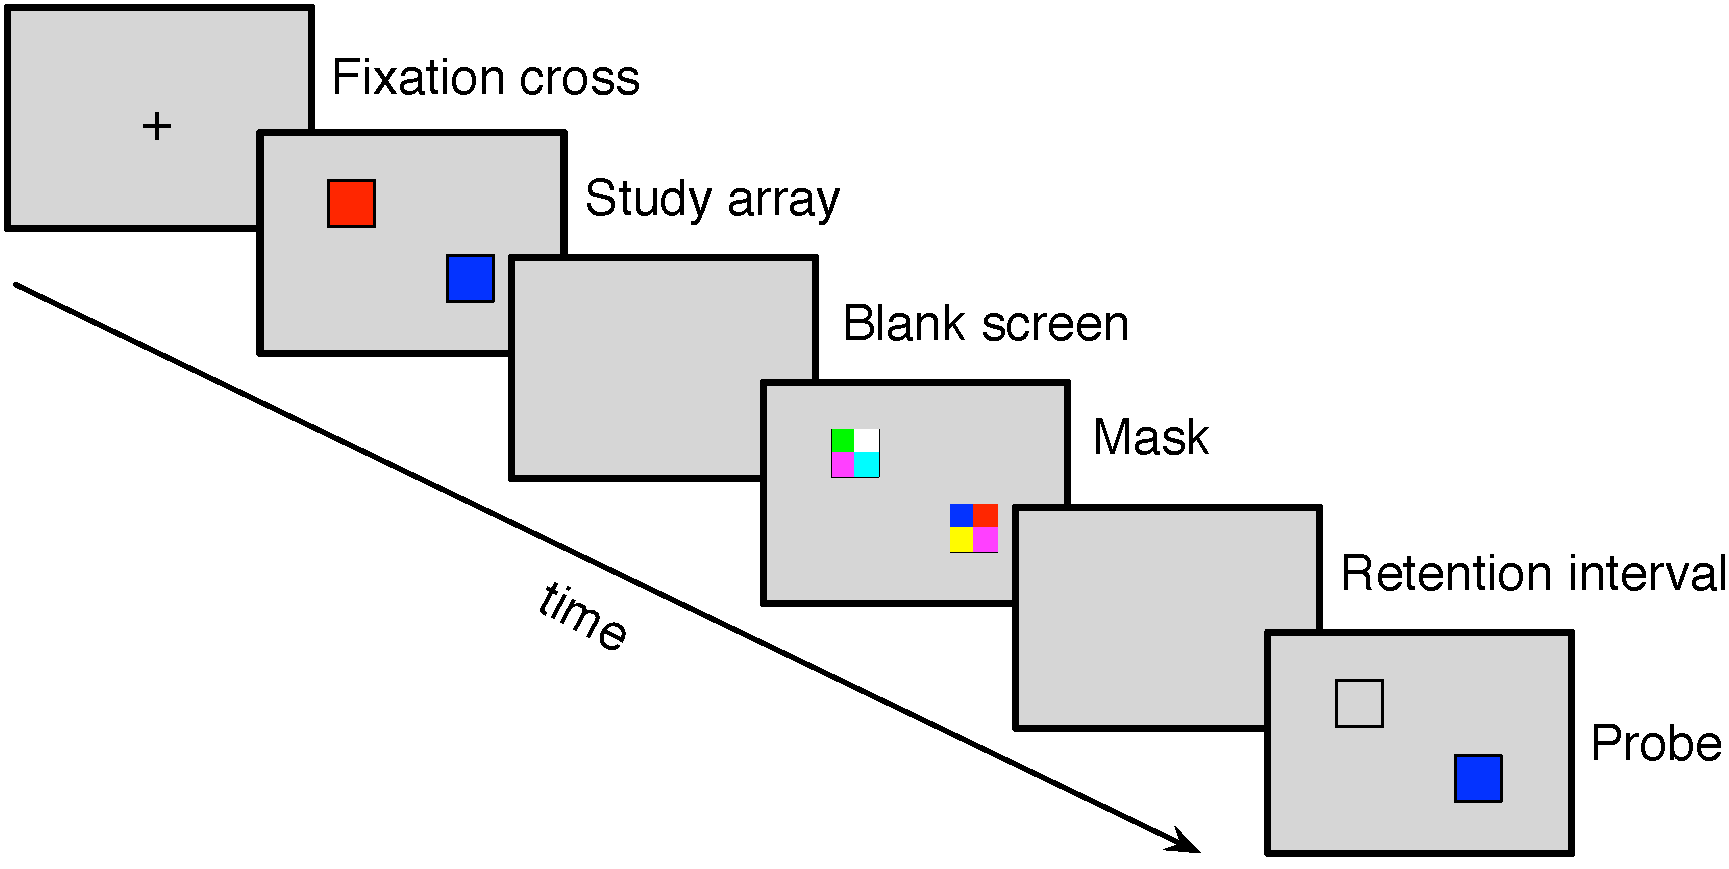
\includegraphics[width=0.5\textwidth]{figures/paradigm}
	\caption{A schematic representation of a set size two trial in the simultaneous presentation condition. For the exact timing, please consult the \emph{Procedure} sub-section. Note that the image is not to scale.}

	\label{fig:paradigm}
\end{figure}


The overall structure of the task is depicted in Figure \ref{fig:paradigm}. The trial started with a fixation cross that was on screen for 2,000 \emph{ms}. The study time in the simultaneous block was a linear function of the set size (study time = set size $\times$ 100 \emph{ms}) and the set sizes were 2, 4, and 8. In the sequential block, the stimuli appeared one after another. Each stimulus was shown with a thin, black outline and remained on the screen for 100 \emph{ms}. The stimulus color was then replaced with the background gray color and the black outline remained. After an inter-stimulus interval of 200 \emph{ms} the following stimulus appeared on screen. The outlines of all stimuli remained on screen until a mask appeared. There was a 250 \emph{ms} blank screen between the study array (or the final stimulus color in the sequential presentation) and the mask. The mask was displayed for 500 \emph{ms}. Each individual stimulus mask was made up of a $4 \times 4$ grid of colored rectangles and the colors were randomly chosen from the same color set as the whole array. After the mask disappeared, a 2,250 \emph{ms} retention interval (blank screen) delayed the onset of a single probe. The probe remained on screen until the participant made a response. Alongside the probe were thin, black outlines of the other stimuli from the study array, which were shown to prevent the participant from being unsure about which of the studied stimuli was probed.



\section{Results}
% !TeX root = sta_paper.tex

Prior to data analysis, all trials containing invalid responses (0.1\% of trials) were removed, and trials with unusually long or short response times ($<200ms$ or $>3s$; 2\% of trials) were excluded. The overwhelming majority of these were too slow, possibly because participants took unscheduled breaks by deliberately delaying their response. Overall, 36,495 trials across the 15 participants remained for analysis. Descriptive statistics for task performance across conditions are summarized in Figure \ref{fig:descriptiveStats}. Overall accuracy is high in the set size 2 condition, as expected, and decreases as set size increases. In addition, Table \ref{tab:descriptiveStats} shows the mean hit and false alarm rates across all participants.

\begin{table}[ht]
{
\centering
\begin{tabular}{rrrrr}
  \hline
& \multicolumn{4}{c}{hits}\\
  \hline
& \multicolumn{2}{c}{simultaneous} & \multicolumn{2}{c}{sequential} \\
 set size & articulate & silent & articulate & silent \\ 
  \hline
  2 & 0.95 (0.022) & 0.95 (0.036) & 0.94 (0.026) & 0.94 (0.032) \\ 
  4 & 0.84 (0.065) & 0.88 (0.063) & 0.82 (0.076) & 0.82 (0.097) \\ 
  8 & 0.72 (0.079) & 0.70 (0.100) & 0.70 (0.101) & 0.70 (0.174) \\ 
  \hline
 & \multicolumn{4}{c}{false alarms}\\
  \hline
& \multicolumn{2}{c}{simultaneous} & \multicolumn{2}{c}{sequential}\\
set size & articulate & silent & articulate & silent \\ 
  \hline
  2 & 0.08 (0.040) & 0.06 (0.035) & 0.11 (0.066) & 0.07 (0.039) \\
  4 & 0.25 (0.131) & 0.22 (0.132) & 0.31 (0.166) & 0.26 (0.154) \\
  8 & 0.41 (0.120) & 0.39 (0.138) & 0.41 (0.142) & 0.42 (0.159) \\
\hline
\end{tabular}
}
\caption{Mean hit and false alarm rates for all conditions across all participants. Numbers in parentheses are standard deviations of the corresponding means.} 
\label{tab:descriptiveStats}
\end{table}

\begin{figure}[t]
 	\centering
	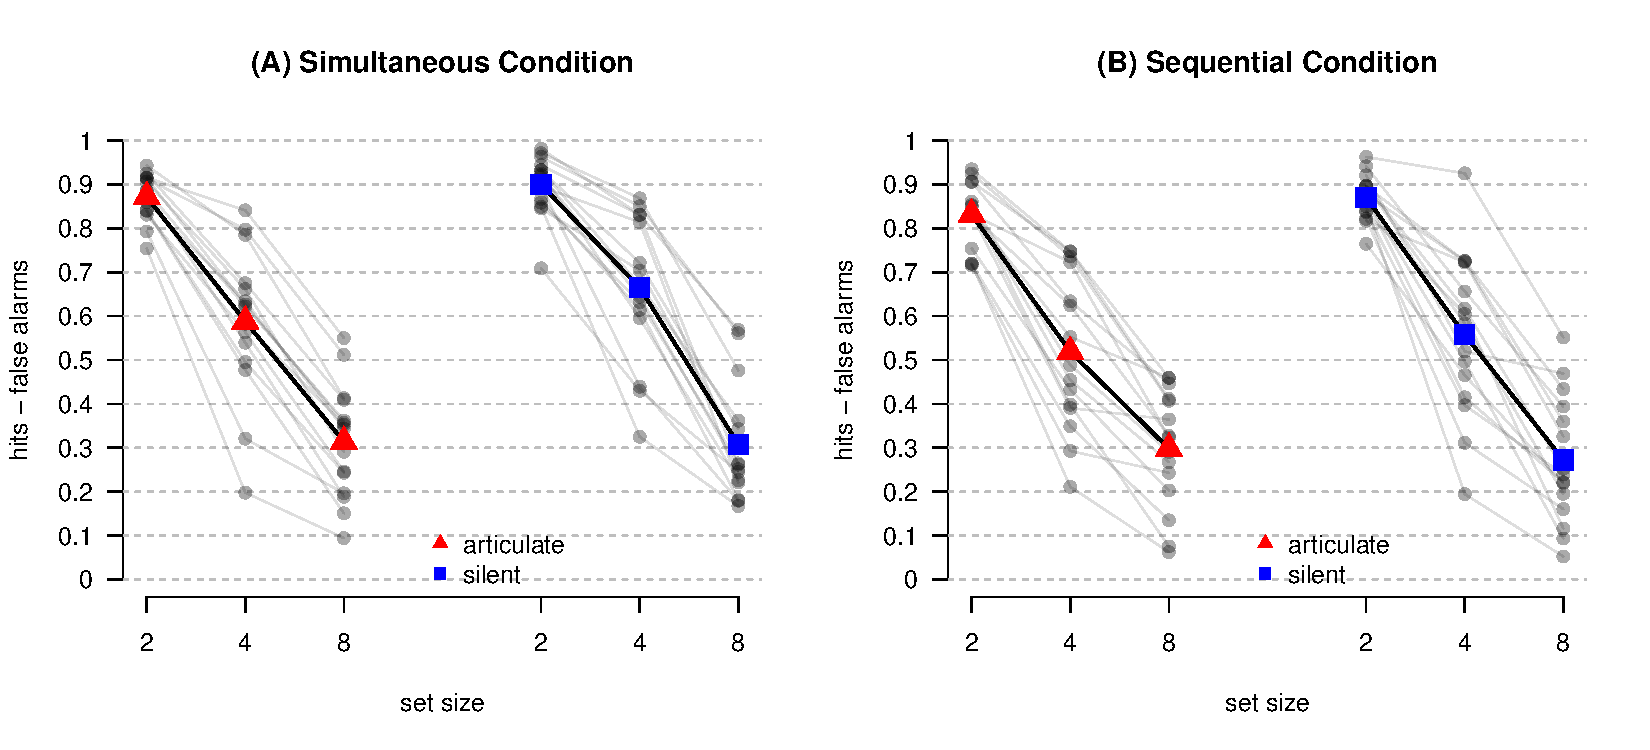
\includegraphics[width=\textwidth]{figures/descriptiveStats}
	\caption{Descriptive statistics for the relevant performance measure $d$ across the different conditions of the experiment. Semi-transparent black circles show the mean performance in each condition per participant and lines connect individual participants' means. Larger, colored symbols are group means for each condition, connected by thicker, black lines.}

	\label{fig:descriptiveStats}
\end{figure}


In order to assess the performance while controlling for response bias, for each condition-participant-set size combination we subtracted the false alarm rate from the hit rate to form an overall performance measure $d$ \citep{Cowan:etal:2005,Rouder:etal:2011}. Of particular interest is how the performance advantage for the silent condition is affected by the type of presentation. If participants verbalize when the presentation is sequential, we would predict that articulation would hurt performance much more with sequential presentation, and thus the advantage for the silent condition would be larger with sequential presentation. Figure~\ref{fig:effects}A plots the silent advantage in the simultaneous condition as a function of the same for the sequential condition for all participant by set size combinations. If participants were verbalizing, we would predict that many points would fall below the diagonal, indicating a greater advantage in the sequential condition. However, 27 out of the 45 points actually fall {\em above} the diagonal, inconsistent with the verbalization hypothesis. 

We also examined whether the apparent lack of an effect may be due to differences in strategy over the experimental sessions; however, a similar picture emerges when the effect is examined across the time, as in Figure~\ref{fig:effects}B. The verbalization hypothesis would predict that points would fall above the horizontal line at 0; on average; however, if anything, the points tend to fall {\em below} the line.

\begin{figure}[t]
 	\centering
	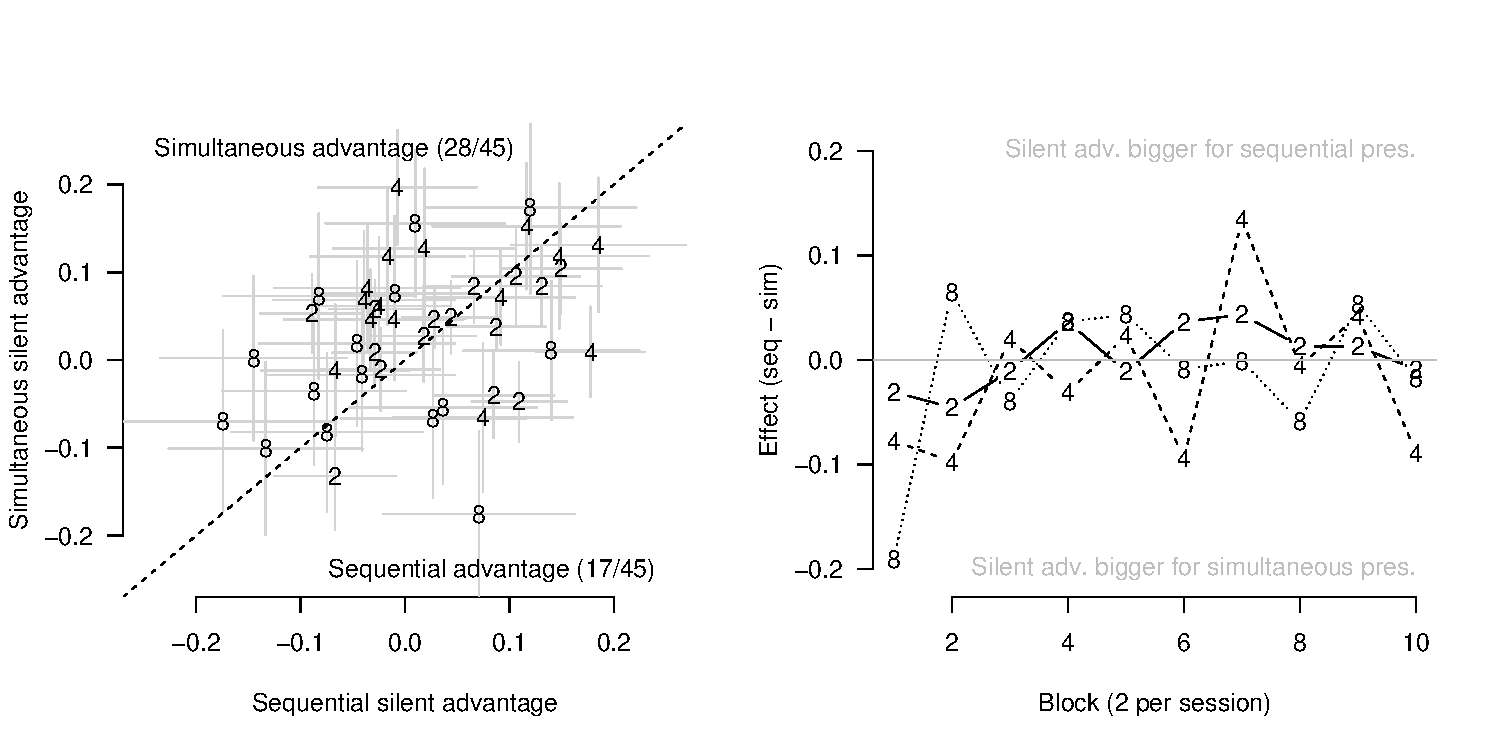
\includegraphics[width=\textwidth]{figures/effects}
	\caption{A: Advantage for silent condition (i.e., $d$ in silent condition minus $d$ in articulate condition) with simultaneous presentation as a function of the same for sequential presentation. Each point represents a single participant and set size. Error bars are approximate standard errors. B: The difference between the advantage for the silent condition in the sequential and simultaneous presentation conditions as a function of experimental block. In both plots, the number for each point represents the set size.}

	\label{fig:effects}
\end{figure}


\subsection{State-trace analysis}
Another way to examine whether there is any evidence for verbalization is a {\em state-trace analysis}. State-trace analysis, outlined in its original form by \citet{Bamber:1979}, is a data analysis technique intended to reveal how many latent dimensions a system requires to produce observed empirical results. A simple system may have only one latent dimension (e.g., memory capacity), and all experimental manipulations affect performance along that latent dimension. More complex systems may show relationships that are impossible to explain by a single dimension, and hence require positing more latent constructs. Considering visual change detection performance, one might imagine that only one latent dimension (e.g. visual memory capacity) or two latent dimensions (e.g. visual and verbal memory capacity) contribute to recognition accuracy. Articulatory suppression would only be necessary if there is an additional latent dimension that relies on verbal resources. That is, if visual change detection performance can be explained by a single latent dimension then articulatory suppression is not needed. To see whether a single latent dimension is supported, it is necessary to compare typical visual change detection accuracy to detection accuracy in a situation where verbal recoding would be especially beneficial, and compare the effect of preventing verbal recoding across these scenarios. 

In the logic of state-trace analysis, performance in the sequential and simultaneous presentation conditions arise from either one or more latent constructs. If they both arise from a single latent variable, such as working memory capacity --- and if performance in both is a monotone function of the latent variable -- then performance in the sequential presentation must be a monotone function of performance in the simultaneous condition. To the extent to which no monotone function can describe the relationship between simultaneous and sequential task performance, two latent constructs --- perhaps visual and verbal working memory capacity --- are assumed to be needed to describe the performance.

For the state-trace analysis, we again used $d$, the hit rate minus the false alarm rate, as a measure of performance. To reduce possibly spurious deviations we computed Bayesian estimates of $d$ under three reasonable constraints: first, we assumed that the true hit rate was greater than the true false alarm rate, and thus performance was truly above chance. Second, for both the sequential and the simultaneous condition, $d$ must decrease with increasing array set size; for instance, true $d$ to a set size of 8 cannot be better than performance to set size 4, all other things being equal. Third, it was assumed that suppression cannot benefit performance; for each set size and presentation condition, the true $d$ in the articulate condition must be less than in the silent condition. This restriction was applied because a small dual-task cost appearing in all conditions would be consistent within any working memory theory, and with our stimuli and meaningless articulation instructions, no benefit of articulation was reasonably expected. Estimating the true discrimination under these restrictions yields a less error-prone measure of performance due to the exclusion of implausible data patterns. 

%%% full-page figure
\begin{figure}
 	\centering
	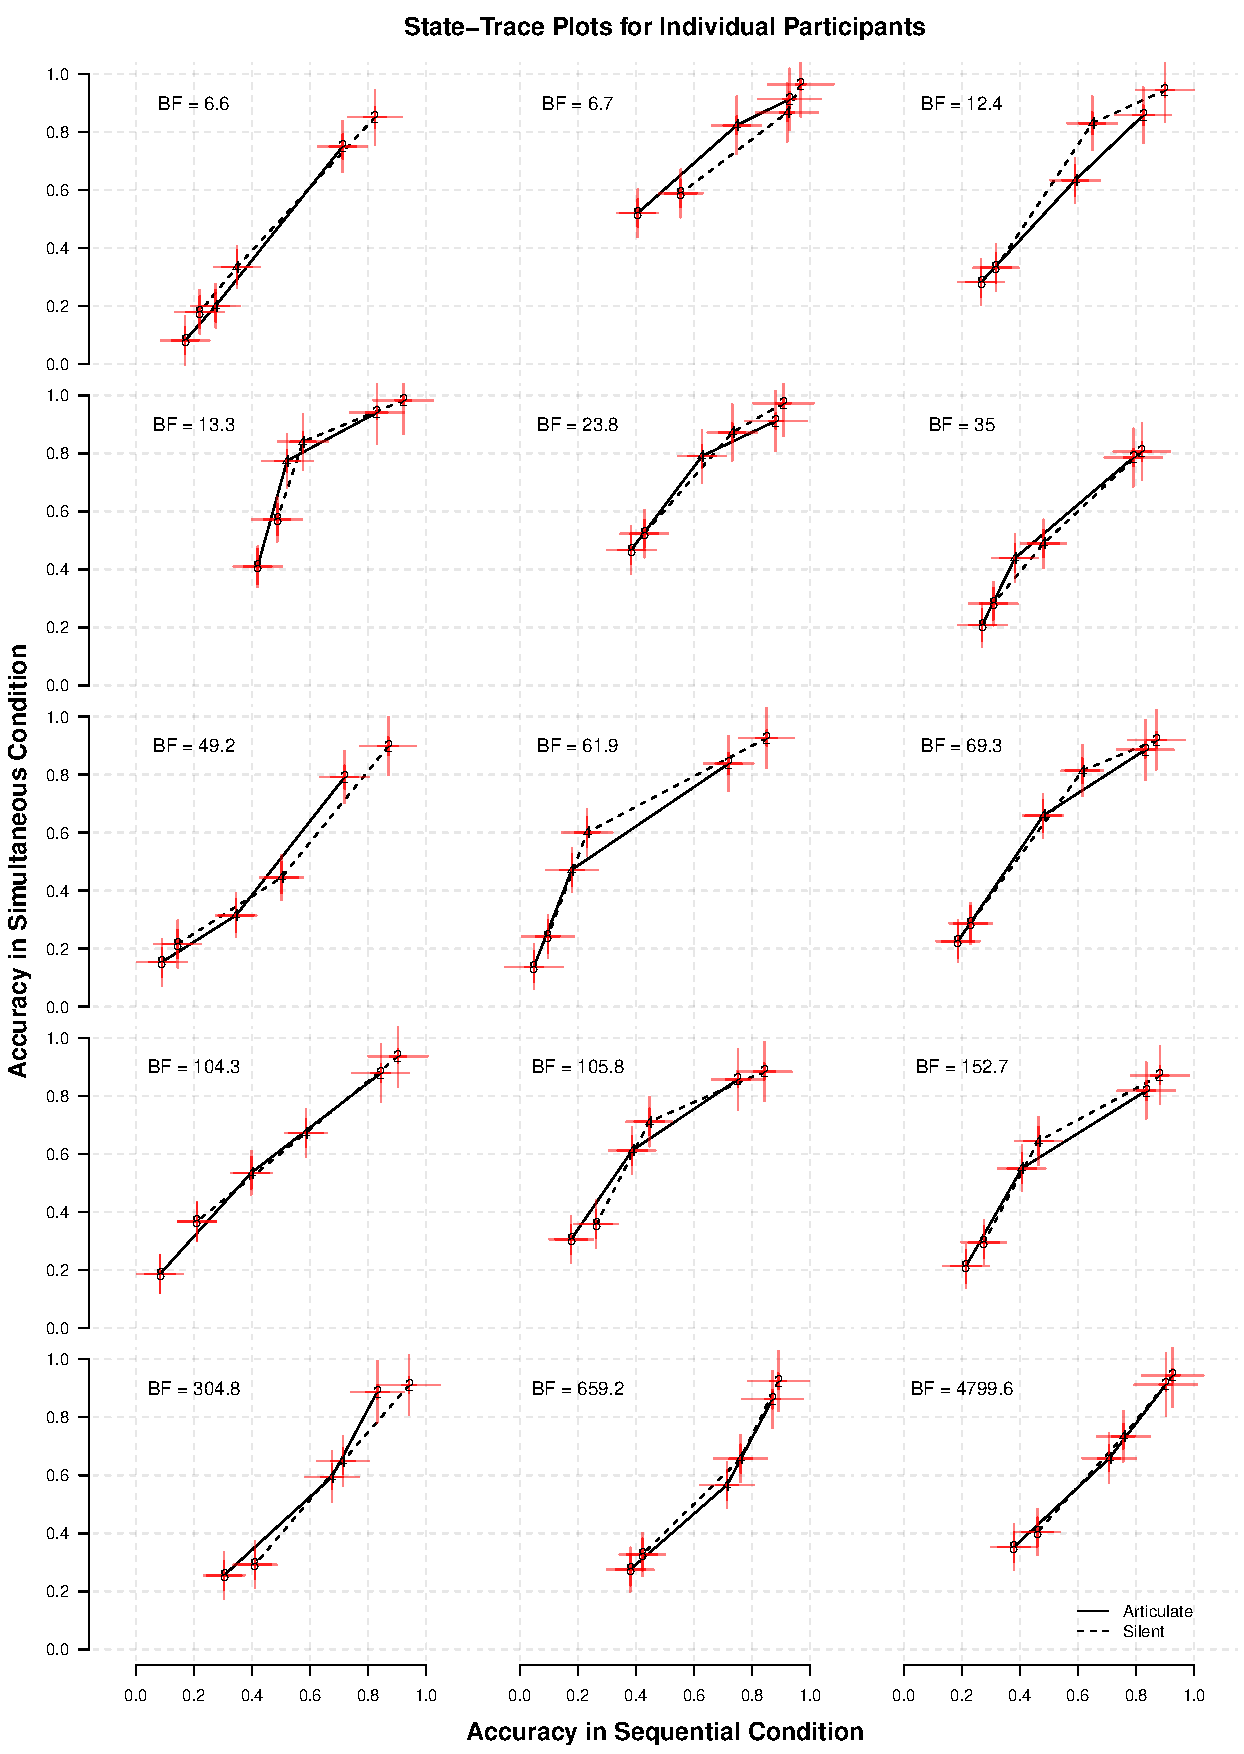
\includegraphics[width=\textwidth]{figures/grid_plot_v2}
	\caption{Individual state-trace plots for the 15 participants. The dependent variables are hit rate minus false alarm rate $d$ for the three set sizes (2, 4, and 8)  and are plotted with standard errors. In the top left corner, individual plot also features the Bayes factor in favor of a monotone ordering of the points over a non-monotone ordering.}

	\label{fig:ST_plots}
\end{figure}

Figure~\ref{fig:ST_plots} shows the state-trace plots for each participant, formed by plotting estimated performance in the simultaneous presentation condition against the performance in the sequential condition. State-trace logic says that more than one latent construct is needed to explain the data to the extent that these points cannot be joined by a single, monotone curve; however, as can be seen from the state-trace plots for all participants, the state-trace plots are strikingly monotone. There does not appear to be any evidence that more than a single latent construct --- (visual) working memory capacity --- is needed, and thus no evidence that verbalization plays a role in performance in this task.

One way to quantify the support for monotonicity in the state-trace plots is to compute Bayes factors that compare the evidence for two hypotheses: first, that the true performance underlying the state-trace plots are ordered the same on both axes (that is, they can be described by a monotone curve), and second, that they are not ordered the same on both axes \citep{Prince:etal:2012}. The Bayes factor is a measure of relative support indicating the degree to which the data change the odds favoring one hypothesis over the other. A Bayes factor of 10, for instance, indicates that the data should change the odds in favor of one hypothesis over the other by a factor of 10. If, before observing the data one was equally disposed to the two hypotheses (a relative odds of 1), then after the data, the favored model would be supported by an odds of $10 \times 1 = 10$.  Here, we discuss the numerical values of the Bayes factors without providing details of their calculation. We refer the reader to \citet{Prince:etal:2012} for technical details, and to the supplement to this article for details of how the Bayes factors were computed \citep[see also][]{Davis-Stober:etal:inpress}.

In addition to the state-trace plots for each participant, Figure~\ref{fig:ST_plots} also contains the Bayes factor favoring a monotone ordering of the points over a non-monotone one. The Bayes factors uniformly favor the monotone ordering of the points. The Bayes factors range from about 7 to almost 5000. These data do not appear to provide any evidence for a deviation from monotonicity.


\section{Discussion and Conclusions}
% !TeX root = sta_paper.tex

In this study, the main question was whether verbalization assists with other processes to influence visual memory performance. In that case, the application of articulatory suppression would be required to disengage that dimension so that a pure measure of visual memory performance can be obtained. Neither a straightforward descriptive analysis nor a state-trace analysis revealed evidence that participants engaged in verbalization as a strategy, even though the experimental design favored the use of verbalization even more than typical visual change detection tasks. The lack of a complex relationship between suppression, presentation type, and performance provides evidence that verbal recoding was not a strategy used by the participants in this task.

One caveat for the interpretation of these results is that state-trace analysis, like all methods, is limited by the resolution of the data. Detecting deviations from monotonicity in a curve depends on how finely points on the curve are measured. It is possible that with finer gradations of set size, we might be able to detect non-monotonicities that are not apparent in these data. However, visual inspection of the state-trace plots in Figure~\ref{fig:ST_plots} suggests that whatever effect of articulatory suppression exists is small; detecting such a small deviation from monotonicity would require finer gradations of sets size and more trials per set size. Although a small deviation from monotonicity may in fact exist, it is unlikely to have any substantial effect on measurements of visual working memory capacity.

Stimulus presentation duration is likely a crucial factor determining whether verbalization strategies are employed in visual memory tasks. Another possible reason for the lack of an effect of articulatory suppression might be that the presentation rate in the experiment was rather fast relative to the time it takes to verbalize information. However, the stimulus presentation timings we employed (100 ms) are typical of visual change detection tasks, which range from 8 ms per item \citep{Woodman:Vogel:2005} to as much as 500 ms per item \citep{Brockmole:etal:2008} in the visual change detection papers cited in our Introduction, and the actual time to articulate was closer to 300 ms in our study. For presentations as fast or faster than the 100 ms per item rate that we measured, it appears safe to assume that verbalization does not augment visual change detection performance. The abstractness of the stimuli employed also likely influences the extent to which verbalization occurs. Researchers employing nameable visual stimuli at a pace enabling verbalization should still consider employing precautionary articulatory suppression if their goal is to isolate specifically visual memory. However, based on our data, we conclude that in typical visual change detection, this precaution is unnecessary.

Finally, we emphasize that we do not dispute that verbal processes can in principle be applied to visual stimuli, and likely are under some circumstances \citep[e.g.][]{Brandimonte:etal:1992}. Our manipulations were designed specifically to uncover the extent to which verbalization was likely to influence visual memory performance under the conditions typical to visual change detection tasks. Our findings suggest that participants do not make use of this hypothetical second dimension (i.e., verbalization) in this task context. Consequently, enforcing precautionary articulatory suppression does not seem to be necessary to get interpretable data from visual change detection tasks.


\printbibliography

\end{document}
